\subsection{The addition task}
\begin{frame}{A pathological problem example}
	
	
	An input sequence:
	
	\vspace{1em}
	
	\begin{tabular}{|c|c|c|c|c|c|c|c|c|c}
		\hline  marker & 0&  1&  0&  $\hdots$& 0 & 1 & 0 & 0  \\ 
		value & 0.3&  \textbf{0.7}&  0.1&  $\hdots$& 0.2& \textbf{0.4} & 0.6& 0.9  \\ 
		\hline 
	\end{tabular}
	
	\vspace{1em}
	The predicted output should be the sum of the two one-marked positions (1.1). 
	\pause
	\vspace{1em}
	\begin{block}{Why is this a difficult problem?}
		Because of its long time dependencies.
	\end{block}
	
\end{frame}

\begin{frame}{Vanishing gradient: an illustration}
	\begin{figure}
		\centering
		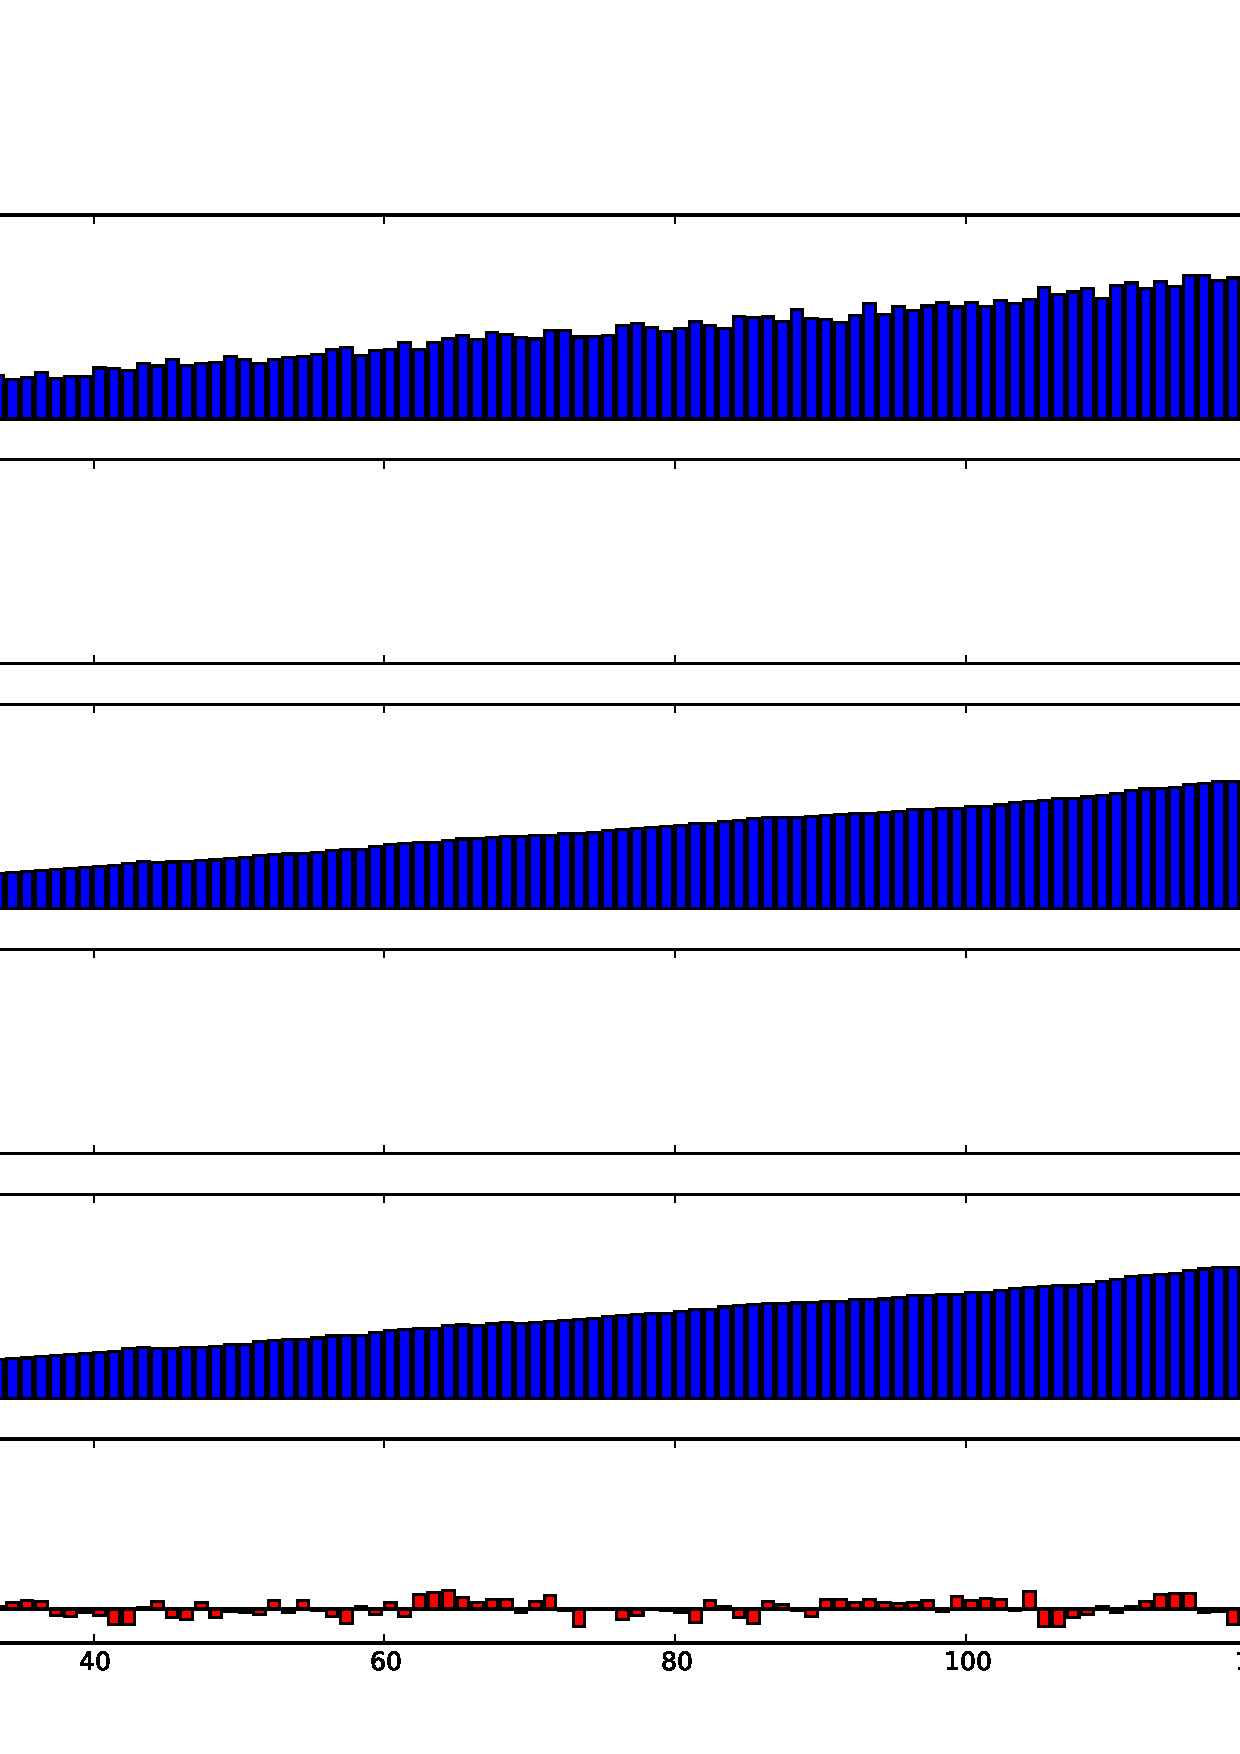
\includegraphics[width=1\textwidth]{temporal_gradients.png}
		\caption{Norm of the temporal gradients at different time steps.}
	\end{figure}
\end{frame}


\subsection{A sufficient condition}
\begin{frame}{Vanishing gradient: a sufficient condition}
	\begin{equation}
	\frac{\partial \vec{a}^t}{\partial \vec{a}^k} = \prod_{i=t-1}^{k}  diag(\sigma'(\vec{a}^i)) \cdot \mat{W}^{rec}.
	\label{eq:temporalComponent}
	\end{equation}
	
	Taking the singular value decomposition of $\mat{W}^{rec}$:
	\begin{equation}
	\mat{W}^{rec} =  \mat{S}\cdot\mat{D}\cdot\mat{V}^T
	\end{equation}
	where $\mat{S},\mat{V}^T$ are squared orthogonal matrices and $\mat{D}\defeq diag(\mu_1, \mu_2,...,\mu_r)$ is the diagonal matrix containing the singular values of $\mat{W}^{rec}$.
	Hence:
	\begin{equation}
	\frac{\partial \vec{a}^t}{\partial \vec{a}^k} = \prod_{i=t-1}^{k}  diag(\sigma'(\vec{a}^i)) \cdot \mat{S}\cdot \mat{D} \cdot \mat{V}^T
	\end{equation}
\end{frame}
\begin{frame}
	Since $\mat{U}$ and $\mat{V}$ are orthogonal matrix, hence $$\norm{\mat{U}}_2=\norm{\mat{V}^T}_2 = 1,$$ and $$\norm{diag(\lambda_1, \lambda_2,...,\lambda_r)}_2 = \lambda_{max},$$ we get
	\begin{align}
	\norm{\frac{\partial \vec{a}^t}{\partial \vec{a}^k}}_2 &= \norm{ (\prod_{i=t-1}^{k} diag(\sigma'(\vec{a}^i)) \cdot \mat{S}\cdot \mat{D} \cdot \mat{V}^T)}_2\\
	&\leq (\sigma'_{max} \cdot \mu_{max})^{t-k-1}
	\end{align}
\end{frame}

